% Generated by genfigs.py -- all coordinates computed from the formulas of the paper.
\usepackage{tikz}
\usetikzlibrary{calc,arrows.meta,decorations.pathreplacing}
\definecolor{supp}{RGB}{20,90,160}
\definecolor{trans}{RGB}{30,130,60}
\definecolor{acc}{RGB}{205,95,10}
\definecolor{chainc}{RGB}{150,150,150}
\definecolor{chainp}{RGB}{190,120,120}
\tikzset{
  rect/.style={line width=0.9pt},
  chain/.style={line width=0.4pt,chainc},
  chainpar/.style={line width=0.4pt,chainp},
  support/.style={line width=1.5pt,supp},
  transport/.style={line width=1.1pt,trans},
  accent/.style={line width=1.2pt,acc},
  aux/.style={line width=0.5pt,densely dashed,black!60},
  pt/.style={circle,fill=black,inner sep=1.4pt},
  lab/.style={font=\small,inner sep=2pt},
  ttl/.style={font=\small\bfseries,anchor=west},
  dim/.style={line width=0.5pt,{Latex[length=4pt]}-{Latex[length=4pt]}},
}

\newcommand{\figDecentered}{%
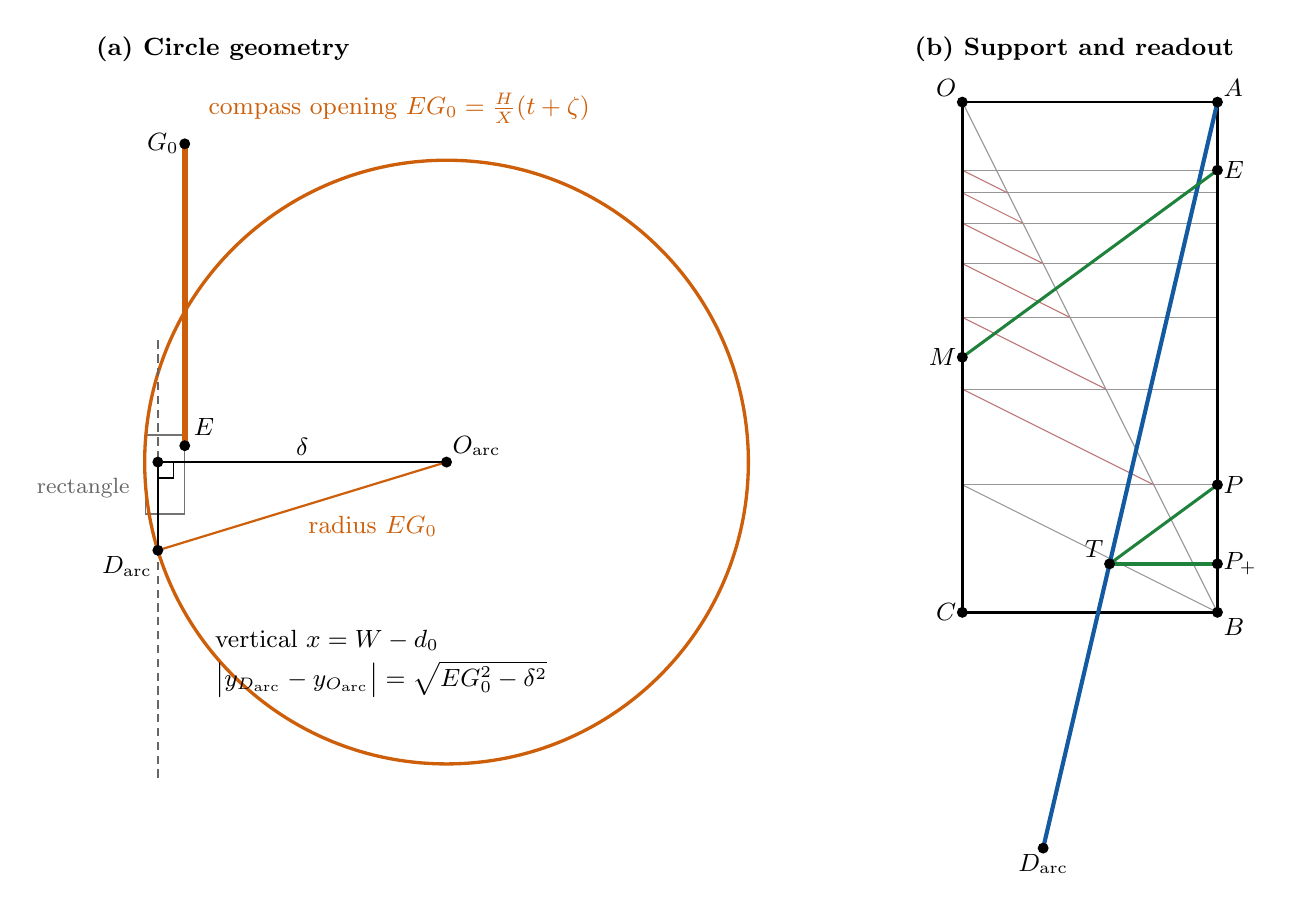
\begin{tikzpicture}[scale=0.25]
\node[ttl] at (-3,23.6) {(a) Circle geometry};
\draw[line width=0.5pt,black!55] (0,0) rectangle (2.0,4.0);
\draw[accent] (15.2980,2.6337) circle (15.3339);
\draw[aux] (0.6337,-13.4)--(0.6337,9.0);
\draw[accent,line width=2.2pt] (2.0000,3.4661)--(2.0000,18.8000);
\draw[line width=0.8pt] (0.6337,-1.8484)--(0.6337,2.6337)--(15.2980,2.6337);
\draw[line width=0.8pt,acc] (15.2980,2.6337)--(0.6337,-1.8484);
\draw[line width=0.5pt] (0.6337,1.8337)-|(1.4337,2.6337);
\node[pt] at (2.0000,18.8000) {};
\node[pt] at (2.0000,3.4661) {};
\node[pt] at (15.2980,2.6337) {};
\node[pt] at (0.6337,-1.8484) {};
\node[pt] at (0.6337,2.6337) {};
\node[lab,left] at (2.0000,18.8000) {$G_0$};
\node[lab,anchor=south west] at (2.1500,3.6661) {$E$};
\node[lab,above right] at (15.2980,2.6337) {$O_{\mathrm{arc}}$};
\node[lab,below left] at (0.6337,-1.8484) {$D_{\mathrm{arc}}$};
\node[lab,anchor=west,acc] at (2.9000,20.6) {compass opening $EG_0=\frac HX(t+\zeta)$};
\node[lab,above] at (7.9659,2.6337) {$\delta$};
\node[lab,anchor=north west,acc] at (7.9659,0.1927) {radius $EG_0$};
\node[lab,anchor=north west,align=left] at (3.2337,-5.6) {vertical $x=W-d_0$\\[3pt]$\bigl|y_{D_{\mathrm{arc}}}-y_{O_{\mathrm{arc}}}\bigr|=\sqrt{EG_0^{2}-\delta^{2}}$};
\node[font=\footnotesize,black!60,anchor=east] at (-0.3,1.3) {rectangle};
\begin{scope}[shift={(41.5,-5.0)},scale=6.48]
\node[ttl] at (-0.45,4.4136) {(b) Support and readout};
\draw[chain] (0.0000,4.0000)--(2.0000,0.0000);
\draw[chain] (0.0000,1.0000)--(2.0000,0.0000);
\draw[chain] (0,1.0000)--(2.0,1.0000);
\draw[chain] (0,1.7500)--(2.0,1.7500);
\draw[chain] (0,2.3125)--(2.0,2.3125);
\draw[chain] (0,2.7344)--(2.0,2.7344);
\draw[chain] (0,3.0508)--(2.0,3.0508);
\draw[chain] (0,3.2881)--(2.0,3.2881);
\draw[chain] (0,3.4661)--(2.0,3.4661);
\draw[chainpar] (1.5000,1.0000)--(0.0000,1.7500);
\draw[chainpar] (1.1250,1.7500)--(0.0000,2.3125);
\draw[chainpar] (0.8438,2.3125)--(0.0000,2.7344);
\draw[chainpar] (0.6328,2.7344)--(0.0000,3.0508);
\draw[chainpar] (0.4746,3.0508)--(0.0000,3.2881);
\draw[chainpar] (0.3560,3.2881)--(0.0000,3.4661);
\draw[rect] (0.0000,0.0000) rectangle (2.0000,4.0000);
\draw[support] (2.0000,4.0000)--(0.6337,-1.8484);
\draw[transport] (0.0000,2.0000)--(2.0000,3.4661);
\draw[transport] (2.0000,1.0000)--(1.1543,0.3801);
\draw[transport,line width=1.5pt] (1.1543,0.3801)--(2.0000,0.3801);
\node[lab,above left] at (0.0000,4.0000) {$O$};
\node[lab,above right] at (2.0000,4.0000) {$A$};
\node[lab,left] at (0.0000,0.0000) {$C$};
\node[lab,below right] at (2.0000,0.0000) {$B$};
\node[pt] at (0.0000,4.0000) {};
\node[pt] at (2.0000,4.0000) {};
\node[pt] at (0.0000,0.0000) {};
\node[pt] at (2.0000,0.0000) {};
\node[pt] at (0.0000,2.0000) {};
\node[pt] at (2.0000,3.4661) {};
\node[pt] at (2.0000,1.0000) {};
\node[pt] at (1.1543,0.3801) {};
\node[pt] at (2.0000,0.3801) {};
\node[lab,left] at (0.0000,2.0000) {$M$};
\node[lab,right] at (2.0000,3.4661) {$E$};
\node[lab,right] at (2.0000,1.0000) {$P$};
\node[lab,right] at (2.0000,0.3801) {$P_+$};
\node[lab,above left] at (1.1543,0.3801) {$T$};
\node[pt] at (0.6337,-1.8484) {};
\node[lab,below] at (0.6337,-1.8484) {$D_{\mathrm{arc}}$};
\end{scope}
\end{tikzpicture}%
}

\newcommand{\figMeans}{%
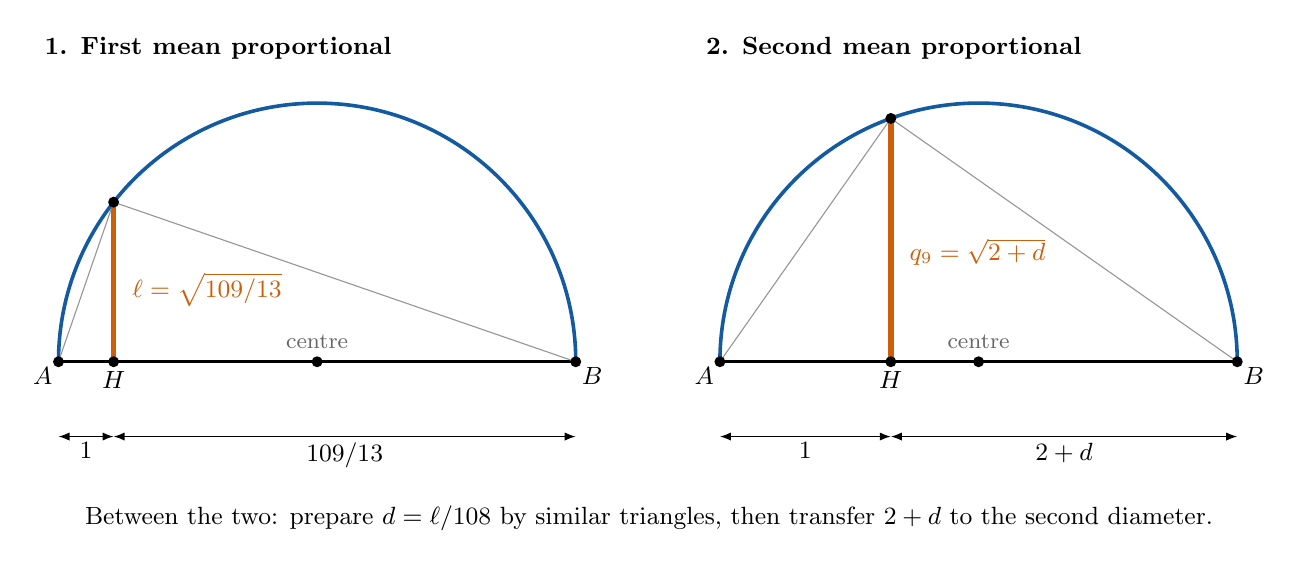
\begin{tikzpicture}
\draw[line width=1.3pt,supp] (6.5692,0) arc (0:180:3.2846);
\draw[rect] (0.0000,0)--(6.5692,0);
\draw[chain] (0.0000,0)--(0.7000,2.0269)--(6.5692,0);
\draw[accent,line width=2pt] (0.7000,0)--(0.7000,2.0269);
\node[pt] at (0.0000,0.0000) {};
\node[pt] at (0.7000,0.0000) {};
\node[pt] at (6.5692,0.0000) {};
\node[pt] at (0.7000,2.0269) {};
\node[pt] at (3.2846,0.0000) {};
\node[lab,below left] at (0.0000,0) {$A$};
\node[lab,below] at (0.7000,-0.05) {$H$};
\node[lab,below right] at (6.5692,0) {$B$};
\node[font=\footnotesize,black!60,above] at (3.2846,0.05) {centre};
\draw[dim] (0.0000,-0.95)--(0.7000,-0.95) node[midway,below,lab] {$1$};
\draw[dim] (0.7000,-0.95)--(6.5692,-0.95) node[midway,below,lab] {$109/13$};
\node[lab,acc,anchor=west,fill=white,inner sep=1.5pt] at (0.8800,0.9121) {$\ell=\sqrt{109/13}$};
\node[ttl] at (-0.3000,3.9846) {1. First mean proportional};
\draw[line width=1.3pt,supp] (14.9700,0) arc (0:180:3.2850);
\draw[rect] (8.4000,0)--(14.9700,0);
\draw[chain] (8.4000,0)--(10.5706,3.0902)--(14.9700,0);
\draw[accent,line width=2pt] (10.5706,0)--(10.5706,3.0902);
\node[pt] at (8.4000,0.0000) {};
\node[pt] at (10.5706,0.0000) {};
\node[pt] at (14.9700,0.0000) {};
\node[pt] at (10.5706,3.0902) {};
\node[pt] at (11.6850,0.0000) {};
\node[lab,below left] at (8.4000,0) {$A$};
\node[lab,below] at (10.5706,-0.05) {$H$};
\node[lab,below right] at (14.9700,0) {$B$};
\node[font=\footnotesize,black!60,above] at (11.6850,0.05) {centre};
\draw[dim] (8.4000,-0.95)--(10.5706,-0.95) node[midway,below,lab] {$1$};
\draw[dim] (10.5706,-0.95)--(14.9700,-0.95) node[midway,below,lab] {$2+d$};
\node[lab,acc,anchor=west,fill=white,inner sep=1.5pt] at (10.7506,1.3906) {$q_9=\sqrt{2+d}$};
\node[ttl] at (8.1000,3.9850) {2. Second mean proportional};
\node[lab,anchor=north,align=center] at (7.5,-1.75) {Between the two: prepare $d=\ell/108$ by similar triangles, then transfer $2+d$ to the second diameter.};
\end{tikzpicture}%
}

\newcommand{\figSupport}{%
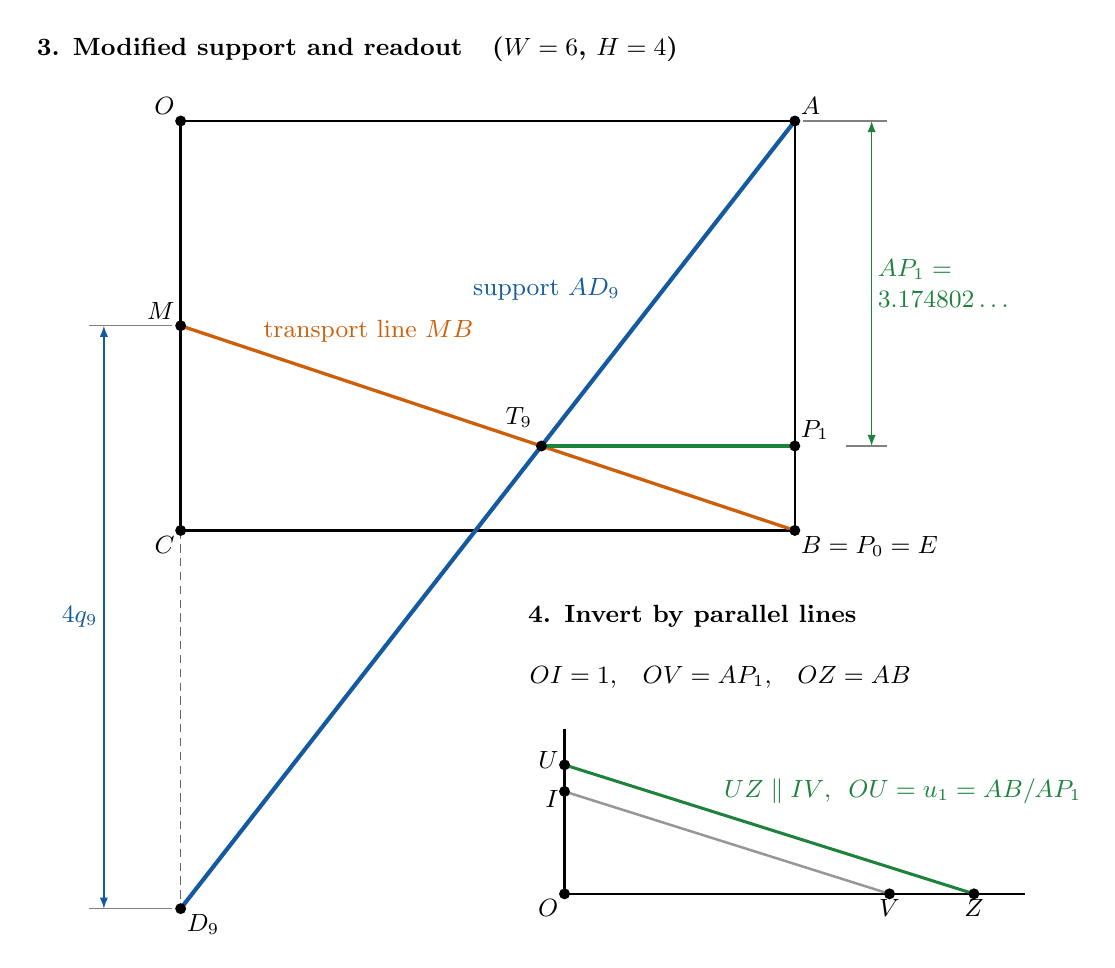
\begin{tikzpicture}[scale=1.3]
\node[ttl] at (-1.5,4.7) {3. Modified support and readout\quad($W=6$, $H=4$)};
\draw[rect] (0.0000,0.0000) rectangle (6.0000,4.0000);
\draw[aux] (0.0000,0.0000)--(0.0000,-3.6946);
\draw[accent] (0.0000,2.0000)--(6.0000,0.0000);
\draw[support] (6.0000,4.0000)--(0.0000,-3.6946);
\draw[transport,line width=1.6pt] (3.5244,0.8252)--(6.0000,0.8252);
\node[pt] at (0.0000,4.0000) {};
\node[pt] at (6.0000,4.0000) {};
\node[pt] at (0.0000,0.0000) {};
\node[pt] at (6.0000,0.0000) {};
\node[pt] at (0.0000,2.0000) {};
\node[pt] at (0.0000,-3.6946) {};
\node[pt] at (3.5244,0.8252) {};
\node[pt] at (6.0000,0.8252) {};
\node[lab,above left] at (0.0000,4.0000) {$O$};
\node[lab,above right] at (6.0000,4.0000) {$A$};
\node[lab,below left] at (0.0000,0.0000) {$C$};
\node[lab,below right] at (6.0000,0.0000) {$B=P_0=E$};
\node[lab,above left] at (0.0000,2.0000) {$M$};
\node[lab,below right] at (0.0000,-3.6946) {$D_9$};
\node[lab,anchor=south] at (3.3044,0.9452) {$T_9$};
\node[lab,above right] at (6.0000,0.8252) {$P_1$};
\draw[dim,supp] (-0.75,2.0000)--(-0.75,-3.6946) node[midway,left,lab,supp] {$4q_9$};
\draw[line width=0.4pt,black!50] (-0.9,2.0000)--(-0.08,2.0000) (-0.9,-3.6946)--(-0.08,-3.6946);
\draw[dim,trans] (6.75,4.0000)--(6.75,0.8252) node[midway,right,lab,trans,align=left] {$AP_1=$\\$3.174802\ldots$};
\draw[line width=0.4pt,black!50] (6.08,4.0000)--(6.9,4.0000) (6.5,0.8252)--(6.9,0.8252);
\node[lab,supp,anchor=east] at (4.35,2.35) {support $AD_9$};
\node[lab,acc,anchor=south west] at (0.75,1.78) {transport line $MB$};
\begin{scope}[shift={(3.75,-3.55)}]
\node[ttl] at (-0.45,2.7099) {4. Invert by parallel lines};
\node[lab,anchor=west] at (-0.4,2.1099) {$OI=1$,\quad $OV=AP_1$,\quad $OZ=AB$};
\draw[rect] (0,0)--(4.5,0) (0,0)--(0,1.6099);
\draw[chain,line width=0.9pt] (0,1)--(3.1748,0);
\draw[transport] (0,1.2599)--(4,0);
\node[pt] at (0.0000,0.0000) {};
\node[pt] at (0.0000,1.0000) {};
\node[pt] at (0.0000,1.2599) {};
\node[pt] at (3.1748,0.0000) {};
\node[pt] at (4.0000,0.0000) {};
\node[lab,below left] at (0,0) {$O$};
\node[lab,left] at (0,0.93) {$I$};
\node[lab,left] at (0,1.3099) {$U$};
\node[lab,below] at (3.1748,0) {$V$};
\node[lab,below] at (4,0) {$Z$};
\node[lab,anchor=south west,trans] at (1.5,0.82) {$UZ\parallel IV$,\ \ $OU=u_1=AB/AP_1$};
\end{scope}
\end{tikzpicture}%
}

\newcommand{\figSubdivision}{%
\begin{tikzpicture}[scale=2.2]
\draw[line width=1.3pt,supp] (4.0,0) arc (0:180:2.0);
\draw[rect] (0,0)--(4.0,0);
\draw[chain] (0,0)--(1.2,1.8330)--(4.0,0);
\draw[accent,line width=2pt] (1.2,0)--(1.2,1.8330);
\node[pt] at (0.0000,0.0000) {};
\node[pt] at (1.2000,0.0000) {};
\node[pt] at (2.0000,0.0000) {};
\node[pt] at (4.0000,0.0000) {};
\node[pt] at (1.2000,1.8330) {};
\node[lab,below left] at (0,0) {$O$};
\node[lab,below] at (1.2,-0.02) {$T$};
\node[lab,below] at (2.0,-0.02) {$C$};
\node[lab,below right] at (4.0,0) {$S$};
\node[lab,above left] at (1.2,1.8330) {$G$};
\node[lab,acc,anchor=west,fill=white,inner sep=1.5pt] at (1.27,0.7699) {$TG=m=\sqrt{ab}$};
\draw[dim] (0,-0.42)--(1.2,-0.42) node[midway,below,lab] {$a$};
\draw[dim] (1.2,-0.42)--(4.0,-0.42) node[midway,below,lab] {$b$};
\node[anchor=west,align=left,font=\small] at (4.3,1.15) {$\lambda\le\tfrac12:\ (a,b,\lambda)\mapsto(a,\,m,\,2\lambda)$\\[8pt]$\lambda>\tfrac12:\ (a,b,\lambda)\mapsto(m,\,b,\,2\lambda-1)$\\[8pt]gap: $\ b/a\ \mapsto\ \sqrt{b/a}$};
\end{tikzpicture}%
}

\newcommand{\figDepth}{%
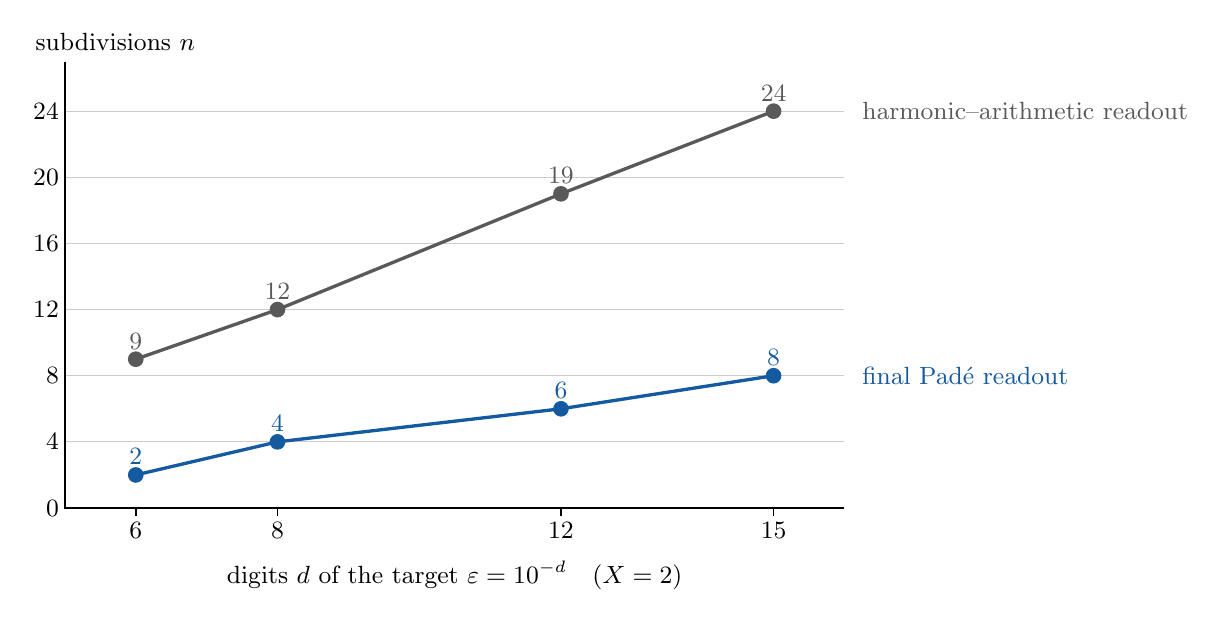
\begin{tikzpicture}
\draw[line width=0.3pt,black!20] (0,0.000)--(9.900,0.000);
\node[lab,left] at (0,0.000) {0};
\draw[line width=0.3pt,black!20] (0,0.840)--(9.900,0.840);
\node[lab,left] at (0,0.840) {4};
\draw[line width=0.3pt,black!20] (0,1.680)--(9.900,1.680);
\node[lab,left] at (0,1.680) {8};
\draw[line width=0.3pt,black!20] (0,2.520)--(9.900,2.520);
\node[lab,left] at (0,2.520) {12};
\draw[line width=0.3pt,black!20] (0,3.360)--(9.900,3.360);
\node[lab,left] at (0,3.360) {16};
\draw[line width=0.3pt,black!20] (0,4.200)--(9.900,4.200);
\node[lab,left] at (0,4.200) {20};
\draw[line width=0.3pt,black!20] (0,5.040)--(9.900,5.040);
\node[lab,left] at (0,5.040) {24};
\draw[rect] (0,5.670)--(0,0)--(9.900,0);
\draw[line width=0.6pt] (0.900,0)--(0.900,-0.1);
\node[lab,below] at (0.900,-0.1) {6};
\draw[line width=0.6pt] (2.700,0)--(2.700,-0.1);
\node[lab,below] at (2.700,-0.1) {8};
\draw[line width=0.6pt] (6.300,0)--(6.300,-0.1);
\node[lab,below] at (6.300,-0.1) {12};
\draw[line width=0.6pt] (9.000,0)--(9.000,-0.1);
\node[lab,below] at (9.000,-0.1) {15};
\draw[line width=1.2pt,black!65] (0.900,1.890)--(2.700,2.520)--(6.300,3.990)--(9.000,5.040);
\node[circle,fill=black!65,inner sep=2pt] at (0.900,1.890) {};
\node[lab,above,black!65] at (0.900,1.940) {9};
\node[circle,fill=black!65,inner sep=2pt] at (2.700,2.520) {};
\node[lab,above,black!65] at (2.700,2.570) {12};
\node[circle,fill=black!65,inner sep=2pt] at (6.300,3.990) {};
\node[lab,above,black!65] at (6.300,4.040) {19};
\node[circle,fill=black!65,inner sep=2pt] at (9.000,5.040) {};
\node[lab,above,black!65] at (9.000,5.090) {24};
\node[lab,black!65,anchor=west] at (10.050,5.040) {harmonic--arithmetic readout};
\draw[line width=1.2pt,supp] (0.900,0.420)--(2.700,0.840)--(6.300,1.260)--(9.000,1.680);
\node[circle,fill=supp,inner sep=2pt] at (0.900,0.420) {};
\node[lab,above,supp] at (0.900,0.470) {2};
\node[circle,fill=supp,inner sep=2pt] at (2.700,0.840) {};
\node[lab,above,supp] at (2.700,0.890) {4};
\node[circle,fill=supp,inner sep=2pt] at (6.300,1.260) {};
\node[lab,above,supp] at (6.300,1.310) {6};
\node[circle,fill=supp,inner sep=2pt] at (9.000,1.680) {};
\node[lab,above,supp] at (9.000,1.730) {8};
\node[lab,supp,anchor=west] at (10.050,1.680) {final Pad\'e readout};
\node[lab,anchor=south west] at (-0.45,5.733) {subdivisions $n$};
\node[lab,anchor=north] at (4.950,-0.6) {digits $d$ of the target $\varepsilon=10^{-d}$\quad($X=2$)};
\end{tikzpicture}%
}

\newcommand{\figAK}{%
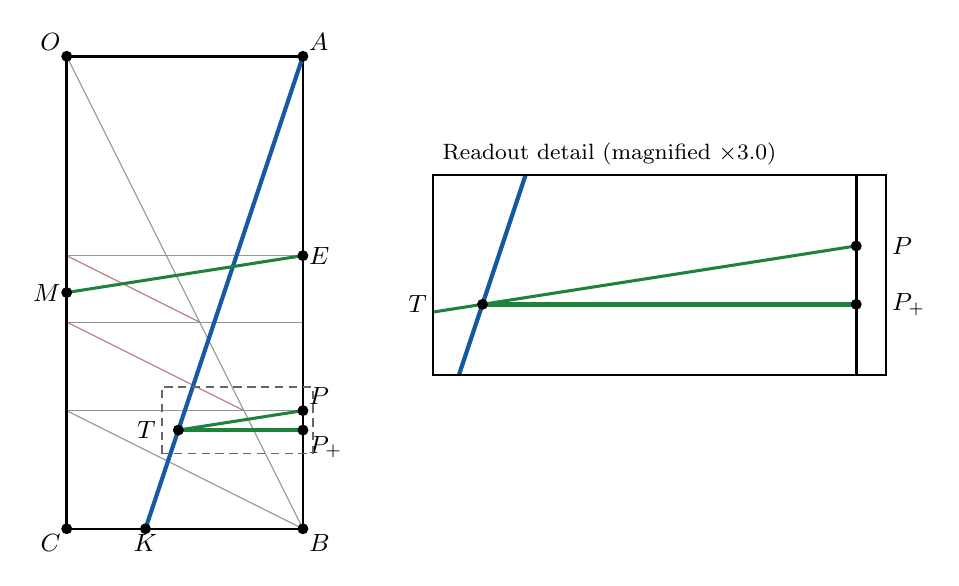
\begin{tikzpicture}[scale=1.5]
\draw[chain] (0.0000,4.0000)--(2.0000,0.0000);
\draw[chain] (0.0000,1.0000)--(2.0000,0.0000);
\draw[chain] (0,1.0000)--(2.0,1.0000);
\draw[chain] (0,1.7500)--(2.0,1.7500);
\draw[chain] (0,2.3125)--(2.0,2.3125);
\draw[chainpar] (1.5000,1.0000)--(0.0000,1.7500);
\draw[chainpar] (1.1250,1.7500)--(0.0000,2.3125);
\draw[rect] (0.0000,0.0000) rectangle (2.0000,4.0000);
\draw[support] (2.0000,4.0000)--(0.6667,0.0000);
\draw[transport] (0.0000,2.0000)--(2.0000,2.3125);
\draw[transport] (2.0000,1.0000)--(0.9451,0.8352);
\draw[transport,line width=1.5pt] (0.9451,0.8352)--(2.0000,0.8352);
\node[lab,above left] at (0.0000,4.0000) {$O$};
\node[lab,above right] at (2.0000,4.0000) {$A$};
\node[lab,below left] at (0.0000,0.0000) {$C$};
\node[lab,below right] at (2.0000,0.0000) {$B$};
\node[pt] at (0.0000,4.0000) {};
\node[pt] at (2.0000,4.0000) {};
\node[pt] at (0.0000,0.0000) {};
\node[pt] at (2.0000,0.0000) {};
\node[pt] at (0.0000,2.0000) {};
\node[pt] at (2.0000,2.3125) {};
\node[pt] at (2.0000,1.0000) {};
\node[pt] at (0.9451,0.8352) {};
\node[pt] at (2.0000,0.8352) {};
\node[lab,left] at (0.0000,2.0000) {$M$};
\node[lab,right] at (2.0000,2.3125) {$E$};
\node[lab,above right] at (2.0000,1.0000) {$P$};
\node[lab,below right] at (2.0000,0.8352) {$P_+$};
\node[pt] at (0.6667,0.0000) {};
\node[lab,below] at (0.6667,0.0000) {$K$};
\draw[aux] (0.8051,0.6352) rectangle (2.0840,1.2000);
\node[lab,left] at (0.8051,0.8352) {$T$};
\begin{scope}[shift={(0.6848,-0.6055)},scale=3.0]
\begin{scope}
\clip (0.8051,0.6352) rectangle (2.0840,1.2000);
\fill[white] (0.8051,0.6352) rectangle (2.0840,1.2000);
\draw[rect] (2.0,-0.3648)--(2.0,2.2000);
\draw[support] (2.0000,4.0000)--(0.6667,0.0000);
\draw[transport] (2.0000,1.0000)--(-3.0000,0.2188);
\draw[transport,line width=1.6pt] (0.9451,0.8352)--(2.0000,0.8352);
\node[pt] at (2.0000,1.0000) {};
\node[pt] at (0.9451,0.8352) {};
\node[pt] at (2.0000,0.8352) {};
\end{scope}
\draw[line width=0.6pt] (0.8051,0.6352) rectangle (2.0840,1.2000);
\node[lab,right] at (2.0840,1.0000) {$P$};
\node[lab,right] at (2.0840,0.8352) {$P_+$};
\node[lab,left] at (0.8051,0.8352) {$T$};
\node[font=\footnotesize,anchor=south west] at (0.8051,1.2000) {Readout detail (magnified $\times3.0$)};
\end{scope}
\end{tikzpicture}%
}

\newcommand{\figAD}{%
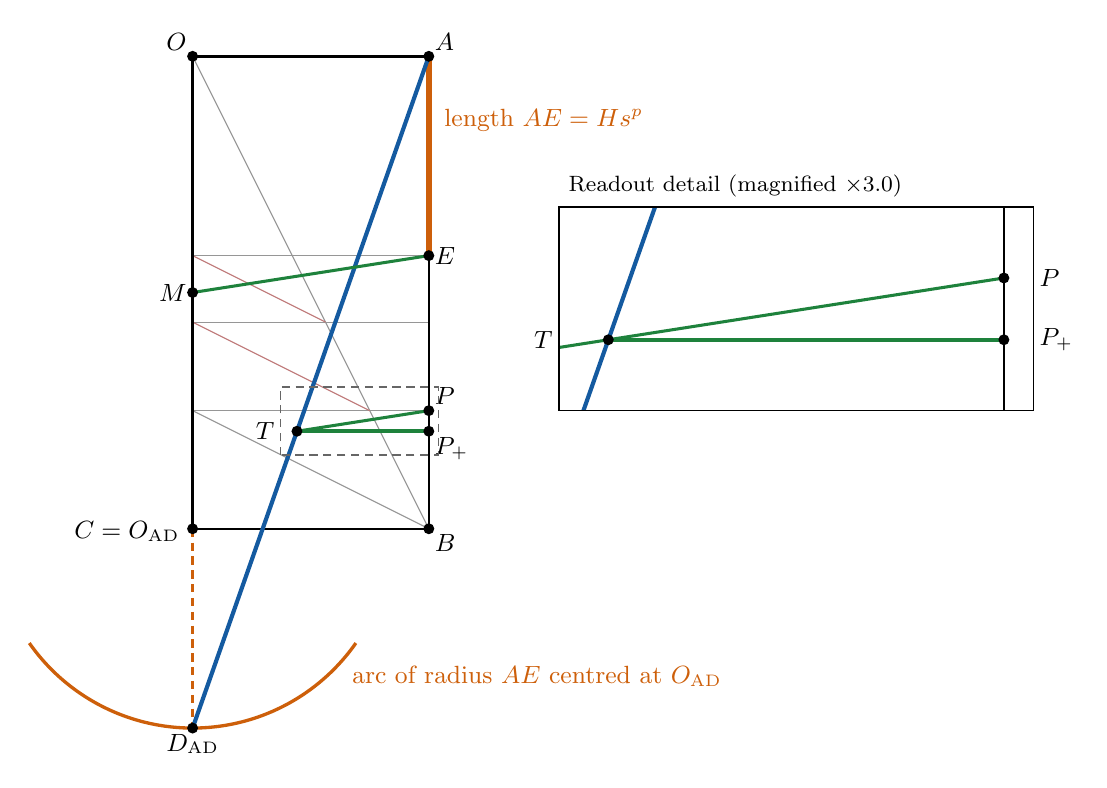
\begin{tikzpicture}[scale=1.5]
\draw[chain] (0.0000,4.0000)--(2.0000,0.0000);
\draw[chain] (0.0000,1.0000)--(2.0000,0.0000);
\draw[chain] (0,1.0000)--(2.0,1.0000);
\draw[chain] (0,1.7500)--(2.0,1.7500);
\draw[chain] (0,2.3125)--(2.0,2.3125);
\draw[chainpar] (1.5000,1.0000)--(0.0000,1.7500);
\draw[chainpar] (1.1250,1.7500)--(0.0000,2.3125);
\draw[rect] (0.0000,0.0000) rectangle (2.0000,4.0000);
\draw[accent] (0.0000,0.0000) ++(215:1.6875) arc (215:325:1.6875);
\draw[accent,densely dashed] (0.0000,0.0000)--(0.0000,-1.6875);
\draw[accent,line width=2.2pt] (2.0000,4.0000)--(2.0000,2.3125);
\draw[support] (2.0000,4.0000)--(0.0000,-1.6875);
\draw[transport] (0.0000,2.0000)--(2.0000,2.3125);
\draw[transport] (2.0000,1.0000)--(0.8837,0.8256);
\draw[transport,line width=1.5pt] (0.8837,0.8256)--(2.0000,0.8256);
\node[lab,above left] at (0.0000,4.0000) {$O$};
\node[lab,above right] at (2.0000,4.0000) {$A$};
\node[lab,anchor=east] at (-0.06,-0.02) {$C=O_{\mathrm{AD}}$};
\node[lab,below right] at (2.0000,0.0000) {$B$};
\node[pt] at (0.0000,4.0000) {};
\node[pt] at (2.0000,4.0000) {};
\node[pt] at (0.0000,0.0000) {};
\node[pt] at (2.0000,0.0000) {};
\node[pt] at (0.0000,2.0000) {};
\node[pt] at (2.0000,2.3125) {};
\node[pt] at (2.0000,1.0000) {};
\node[pt] at (0.8837,0.8256) {};
\node[pt] at (2.0000,0.8256) {};
\node[lab,left] at (0.0000,2.0000) {$M$};
\node[lab,right] at (2.0000,2.3125) {$E$};
\node[lab,above right] at (2.0000,1.0000) {$P$};
\node[lab,below right] at (2.0000,0.8256) {$P_+$};
\node[pt] at (0.0000,-1.6875) {};
\node[lab,below] at (0.0000,-1.6875) {$D_{\mathrm{AD}}$};
\node[lab,acc,anchor=west] at (2.0800,3.4562) {length $AE=Hs^p$};
\node[lab,acc,anchor=west] at (1.3,-1.25) {arc of radius $AE$ centred at $O_{\mathrm{AD}}$};
\draw[aux] (0.7437,0.6256) rectangle (2.0840,1.2000);
\node[lab,left] at (0.7437,0.8256) {$T$};
\begin{scope}[shift={(0.8688,-0.8767)},scale=3.0]
\begin{scope}
\clip (0.7437,0.6256) rectangle (2.0840,1.2000);
\fill[white] (0.7437,0.6256) rectangle (2.0840,1.2000);
\draw[rect] (2.0,-0.3744)--(2.0,2.2000);
\draw[support] (2.0000,4.0000)--(0.0000,-1.6875);
\draw[transport] (2.0000,1.0000)--(-3.0000,0.2188);
\draw[transport,line width=1.6pt] (0.8837,0.8256)--(2.0000,0.8256);
\node[pt] at (2.0000,1.0000) {};
\node[pt] at (0.8837,0.8256) {};
\node[pt] at (2.0000,0.8256) {};
\end{scope}
\draw[line width=0.6pt] (0.7437,0.6256) rectangle (2.0840,1.2000);
\node[lab,right] at (2.0840,1.0000) {$P$};
\node[lab,right] at (2.0840,0.8256) {$P_+$};
\node[lab,left] at (0.7437,0.8256) {$T$};
\node[font=\footnotesize,anchor=south west] at (0.7437,1.2000) {Readout detail (magnified $\times3.0$)};
\end{scope}
\end{tikzpicture}%
}

\newcommand{\figProjective}{%
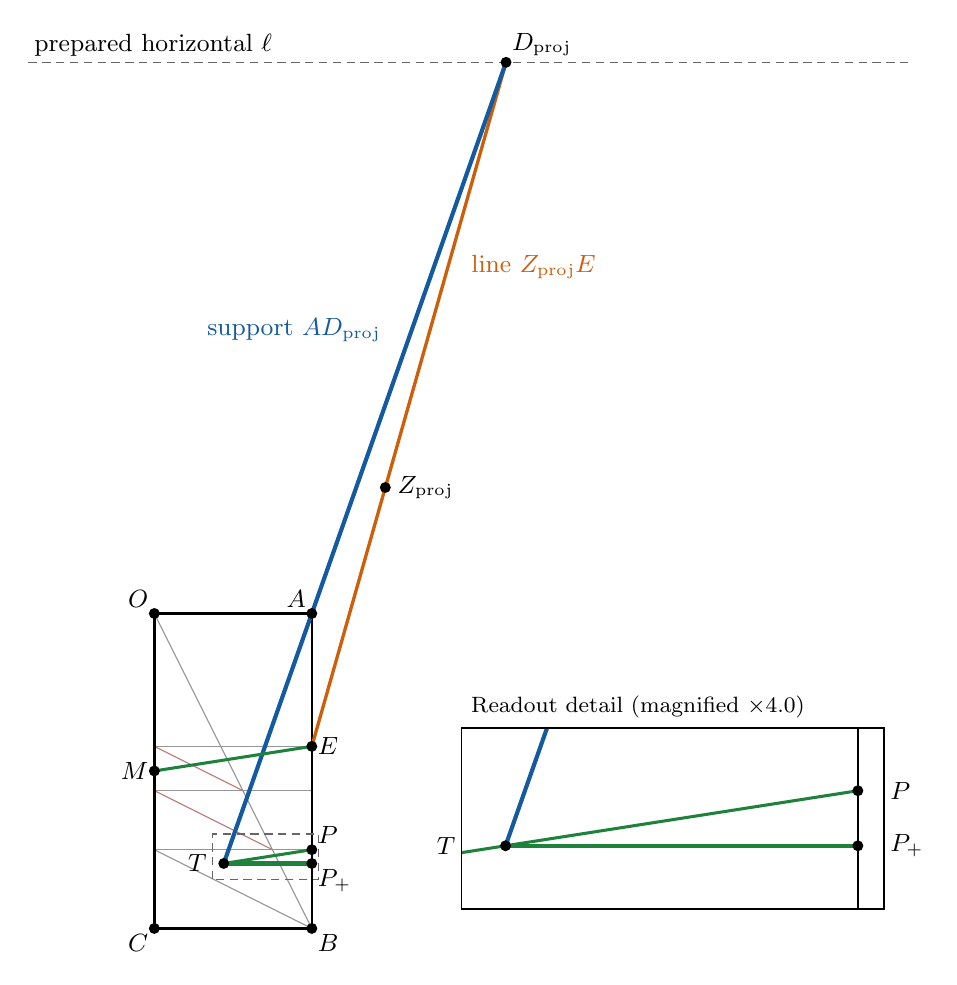
\begin{tikzpicture}[scale=1.0]
\draw[aux] (-1.6,11.0000)--(9.6,11.0000);
\node[lab,anchor=south west] at (-1.6,11.0000) {prepared horizontal $\ell$};
\draw[chain] (0.0000,4.0000)--(2.0000,0.0000);
\draw[chain] (0.0000,1.0000)--(2.0000,0.0000);
\draw[chain] (0,1.0000)--(2.0,1.0000);
\draw[chain] (0,1.7500)--(2.0,1.7500);
\draw[chain] (0,2.3125)--(2.0,2.3125);
\draw[chainpar] (1.5000,1.0000)--(0.0000,1.7500);
\draw[chainpar] (1.1250,1.7500)--(0.0000,2.3125);
\draw[rect] (0.0000,0.0000) rectangle (2.0000,4.0000);
\draw[accent] (2.0000,2.3125)--(4.4664,11.0000);
\draw[support] (0.8814,0.8252)--(4.4664,11.0000);
\draw[transport] (0.0000,2.0000)--(2.0000,2.3125);
\draw[transport] (2.0000,1.0000)--(0.8814,0.8252);
\draw[transport,line width=1.5pt] (0.8814,0.8252)--(2.0000,0.8252);
\node[lab,above left] at (0.0000,4.0000) {$O$};
\node[lab,above left] at (2.0000,4.0000) {$A$};
\node[lab,below left] at (0.0000,0.0000) {$C$};
\node[lab,below right] at (2.0000,0.0000) {$B$};
\node[pt] at (0.0000,4.0000) {};
\node[pt] at (2.0000,4.0000) {};
\node[pt] at (0.0000,0.0000) {};
\node[pt] at (2.0000,0.0000) {};
\node[pt] at (0.0000,2.0000) {};
\node[pt] at (2.0000,2.3125) {};
\node[pt] at (2.0000,1.0000) {};
\node[pt] at (0.8814,0.8252) {};
\node[pt] at (2.0000,0.8252) {};
\node[lab,left] at (0.0000,2.0000) {$M$};
\node[lab,right] at (2.0000,2.3125) {$E$};
\node[lab,above right] at (2.0000,1.0000) {$P$};
\node[lab,below right] at (2.0000,0.8252) {$P_+$};
\node[pt] at (2.9333,5.6000) {};
\node[pt] at (4.4664,11.0000) {};
\node[lab,right] at (3.0133,5.6000) {$Z_{\mathrm{proj}}$};
\node[lab,above right] at (4.4664,11.0000) {$D_{\mathrm{proj}}$};
\node[lab,acc,anchor=west] at (3.95,8.4) {line $Z_{\mathrm{proj}}E$};
\node[lab,supp,anchor=east] at (2.95,7.6) {support $AD_{\mathrm{proj}}$};
\draw[aux] (0.7414,0.6252) rectangle (2.0840,1.2000);
\node[lab,left] at (0.7414,0.8252) {$T$};
\begin{scope}[shift={(0.9345,-2.2509)},scale=4.0]
\begin{scope}
\clip (0.7414,0.6252) rectangle (2.0840,1.2000);
\fill[white] (0.7414,0.6252) rectangle (2.0840,1.2000);
\draw[rect] (2.0,-0.3748)--(2.0,2.2000);
\draw[support] (0.8814,0.8252)--(4.4664,11.0000);
\draw[transport] (2.0000,1.0000)--(-3.0000,0.2188);
\draw[transport,line width=1.6pt] (0.8814,0.8252)--(2.0000,0.8252);
\node[pt] at (2.0000,1.0000) {};
\node[pt] at (0.8814,0.8252) {};
\node[pt] at (2.0000,0.8252) {};
\end{scope}
\draw[line width=0.6pt] (0.7414,0.6252) rectangle (2.0840,1.2000);
\node[lab,right] at (2.0840,1.0000) {$P$};
\node[lab,right] at (2.0840,0.8252) {$P_+$};
\node[lab,left] at (0.7414,0.8252) {$T$};
\node[font=\footnotesize,anchor=south west] at (0.7414,1.2000) {Readout detail (magnified $\times4.0$)};
\end{scope}
\end{tikzpicture}%
}

\newcommand{\figMA}{%
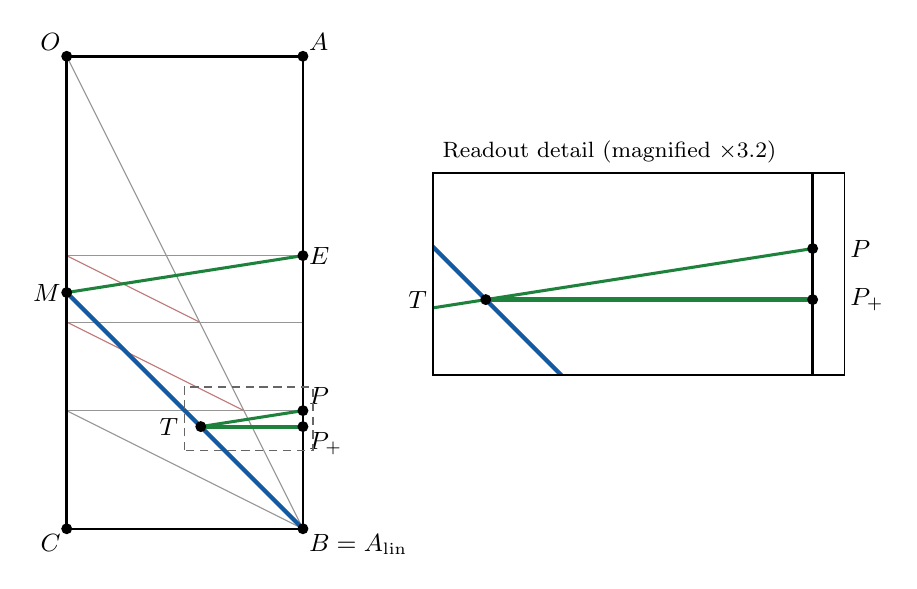
\begin{tikzpicture}[scale=1.5]
\draw[chain] (0.0000,4.0000)--(2.0000,0.0000);
\draw[chain] (0.0000,1.0000)--(2.0000,0.0000);
\draw[chain] (0,1.0000)--(2.0,1.0000);
\draw[chain] (0,1.7500)--(2.0,1.7500);
\draw[chain] (0,2.3125)--(2.0,2.3125);
\draw[chainpar] (1.5000,1.0000)--(0.0000,1.7500);
\draw[chainpar] (1.1250,1.7500)--(0.0000,2.3125);
\draw[rect] (0.0000,0.0000) rectangle (2.0000,4.0000);
\draw[support] (0.0000,2.0000)--(2.0000,0.0000);
\draw[transport] (0.0000,2.0000)--(2.0000,2.3125);
\draw[transport] (2.0000,1.0000)--(1.1351,0.8649);
\draw[transport,line width=1.5pt] (1.1351,0.8649)--(2.0000,0.8649);
\node[lab,above left] at (0.0000,4.0000) {$O$};
\node[lab,above right] at (2.0000,4.0000) {$A$};
\node[lab,below left] at (0.0000,0.0000) {$C$};
\node[lab,below right] at (2.0000,0.0000) {$B=A_{\mathrm{lin}}$};
\node[pt] at (0.0000,4.0000) {};
\node[pt] at (2.0000,4.0000) {};
\node[pt] at (0.0000,0.0000) {};
\node[pt] at (2.0000,0.0000) {};
\node[pt] at (0.0000,2.0000) {};
\node[pt] at (2.0000,2.3125) {};
\node[pt] at (2.0000,1.0000) {};
\node[pt] at (1.1351,0.8649) {};
\node[pt] at (2.0000,0.8649) {};
\node[lab,left] at (0.0000,2.0000) {$M$};
\node[lab,right] at (2.0000,2.3125) {$E$};
\node[lab,above right] at (2.0000,1.0000) {$P$};
\node[lab,below right] at (2.0000,0.8649) {$P_+$};
\draw[aux] (0.9951,0.6649) rectangle (2.0840,1.2000);
\node[lab,left] at (0.9951,0.8649) {$T$};
\begin{scope}[shift={(-0.0844,-0.8276)},scale=3.2]
\begin{scope}
\clip (0.9951,0.6649) rectangle (2.0840,1.2000);
\fill[white] (0.9951,0.6649) rectangle (2.0840,1.2000);
\draw[rect] (2.0,-0.3351)--(2.0,2.2000);
\draw[support] (0.0000,2.0000)--(2.0000,0.0000);
\draw[transport] (2.0000,1.0000)--(-3.0000,0.2188);
\draw[transport,line width=1.6pt] (1.1351,0.8649)--(2.0000,0.8649);
\node[pt] at (2.0000,1.0000) {};
\node[pt] at (1.1351,0.8649) {};
\node[pt] at (2.0000,0.8649) {};
\end{scope}
\draw[line width=0.6pt] (0.9951,0.6649) rectangle (2.0840,1.2000);
\node[lab,right] at (2.0840,1.0000) {$P$};
\node[lab,right] at (2.0840,0.8649) {$P_+$};
\node[lab,left] at (0.9951,0.8649) {$T$};
\node[font=\footnotesize,anchor=south west] at (0.9951,1.2000) {Readout detail (magnified $\times3.2$)};
\end{scope}
\end{tikzpicture}%
}

